\section{计算机的硬件介绍}


%\begin{frame}\ft{\subsecname}
%\begin{figure}
%\centering
%\animategraphics[height=2.in,autoplay,controls,buttonsize=0em,loop]{12}{slide01/images/computer_}{0}{3}
%\end{figure}
%\end{frame}


\begin{frame}\ft{硬件组成}
\begin{itemize}
\item 中央处理器(Central Processing Unit, CPU)\\[0.1in]
\item 存储器\\[0.1in]
  \begin{itemize}
  \item 内存(Memory)\\[0.1in]
  \item 外存:硬盘、U盘\\[0.1in]
  \end{itemize}
\item 输入设备(Input Device):键盘、鼠标、摄像头、扫描仪等\\[0.1in]
\item 输出设备(Output Device):显示器、打印机、音响等
\end{itemize}
\end{frame}


\begin{frame}\ft{主板}
{CPU、内存、硬盘、显卡和声卡等都必须安装在主板上才能运行。}

主板是计算机中最大的一块电路板,是计算机系统中的核心部件,它的上面布满了各种插槽(可连接声卡/显卡/MODEM/等)、接口(可连接鼠标/键盘等)、电子元件,它们都有自己的职责,并把各种周边设备紧紧连接在一起。它的性能好坏对计算机的总体指标将产生举足轻重的影响。
\end{frame}



\begin{frame}[fragile]\ft{主板}
\begin{figure}[h] 
\centering
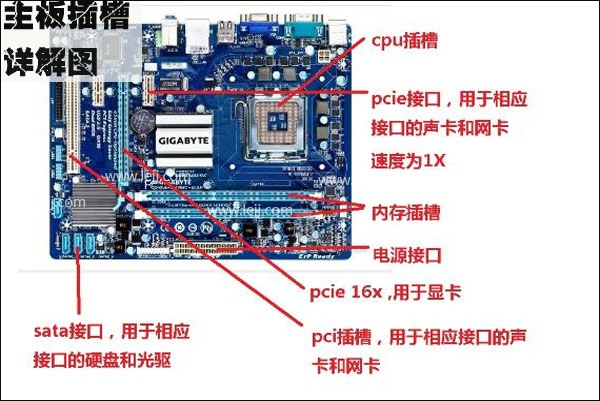
\includegraphics[width=\textwidth]{slide01/images/mobo}
\end{figure}
\end{frame}


\begin{frame}[fragile]\ft{CPU}
\begin{figure}[h] 
\begin{minipage}[t]{0.45\linewidth}
\centering
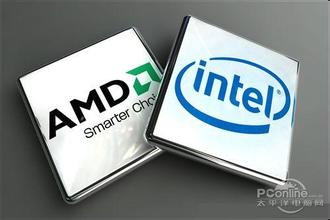
\includegraphics[width=\textwidth]{slide01/images/cpu1}
\end{minipage}
\hfill
\begin{minipage}[t]{0.45\linewidth}
\centering
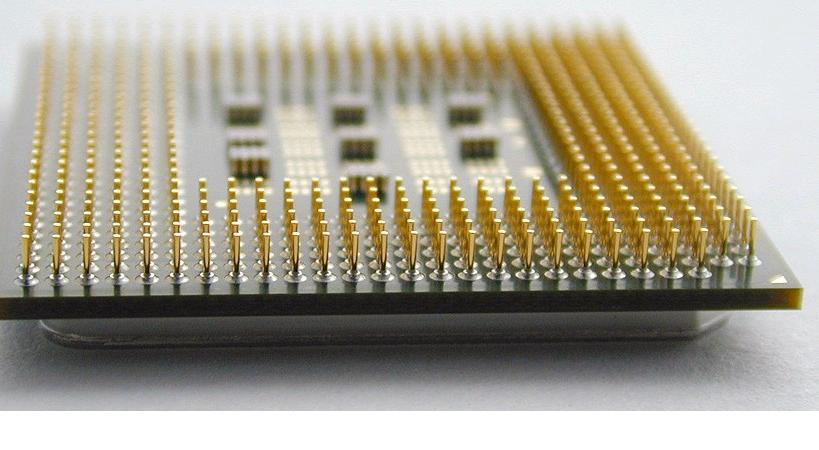
\includegraphics[width=\textwidth]{slide01/images/cpu2}
\end{minipage}
\end{figure}
\end{frame}

\begin{frame}\ft{CPU}
CPU是计算机的大脑,计算机处理数据的能力主要取决于CPU,主要执行以下三种基本操作: 

\begin{itemize}
\item 读出数据:一般从内存读取数据。 \\[0.1in]
\item 处理数据:通过算术逻辑单元对数据进行处理。 \\[0.1in]
\item 写入数据:将数据写入内存。
\end{itemize}

\end{frame}

\begin{frame}\ft{CPU}
 
CPU由运算器、控制器、寄存器和高速缓冲存储器组成。

\end{frame}

\begin{frame}\ft{CPU}
\begin{itemize}
\item  算术逻辑单元(arithmetic logic unit, ALU):负责对数据进行加工处理,包括
\begin{itemize}
\item 算术运算:加、减、乘、除等
\item 逻辑运算:与、或、非、异或、比较等。
\end{itemize} \vspace{.2in}
\item  控制单元(control unit, CU):主要是负责对指令译码,并且发出为完成每条指令所要执行的各个操作的控制信号。\\[0.2in]
\item  \href{https://blog.csdn.net/kwame211/article/details/77773621}{寄存器(register)}:来保存指令执行过程中临时存放的寄存器操作数和中间(或最终)的操作结果。
  \begin{itemize}
  \item 数据寄存器(Data Rigister, DR)
  \item 指令寄存器(Instruction Register, IR)
  \item 程序计数器(Program Counter, PC)
  \item 地址寄存器(Address Register, AR)
  \item 累加寄存器(Accumulator, AC)
  \item 程序状态字寄存器(Program Status Word, PSW)
  \end{itemize}\vspace{0.2in}
% \item 高速缓冲存储器(Cache)\\[0.1in]
%   \begin{itemize}
%   \item 在CPU芯片内,是一个读写速度比内存更快的存储器。
%  \end{itemize}

%当CPU向内存中写入或读出数据时,这个数据也被存储进高速缓冲存储器中。当CPU再次需要这些数据时,CPU就从高速缓冲存储器读取数据,而不是访问较慢的内存,当然,如需要的数据在Cache中没有,CPU会再去读取内存中的数据。
\end{itemize}
\end{frame}
 
\begin{frame}\ft{内存}
\begin{figure}
\centering
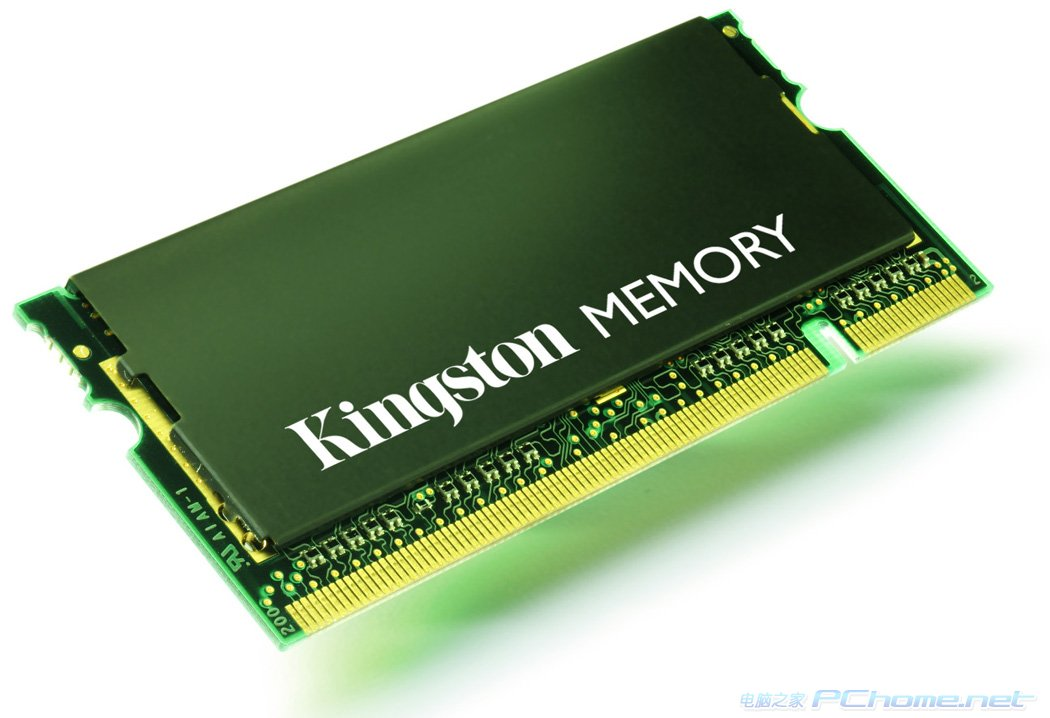
\includegraphics[width=3in]{slide01/images/memory} 
\end{figure}
\end{frame}
 
\begin{frame}\ft{内存}
\begin{itemize}
\item
内存是CPU能直接寻址的存储空间,所有程序的运行都是在内存中进行的。\\[0.1in]
\item
只要计算机在运行中,CPU就会把需要运算的数据调到内存中进行运算,当运算完成后CPU再将结果传送出来。\\[0.1in]
\item
其作用是用于暂时存放CPU中的运算数据,以及与硬盘等外部存储器交换的数据。\\[0.1in]
\end{itemize}
 \end{frame}
 
 \begin{frame}\ft{内存}
 

\begin{itemize}
\item 只读存储器(Read Only Memory, ROM) 
\item[] 只能读取,不能写入,即使断电,存于其中的数据也不会丢失,一般用于存放计算机的基本程序和数据。\\[0.1in] 
\item 随机存储器(Random Access Memory, RAM) 
\item[] 既可读取,也可写入,断电时,存于其中的数据就会丢失。{内存条就是将RAM集成块集中在一起的一小块电路板。}\\[0.2in]

\end{itemize}
 \end{frame}
 
\begin{frame}[fragile]\ft{各类存储器的逻辑连接}
\begin{figure}[h] 
\centering
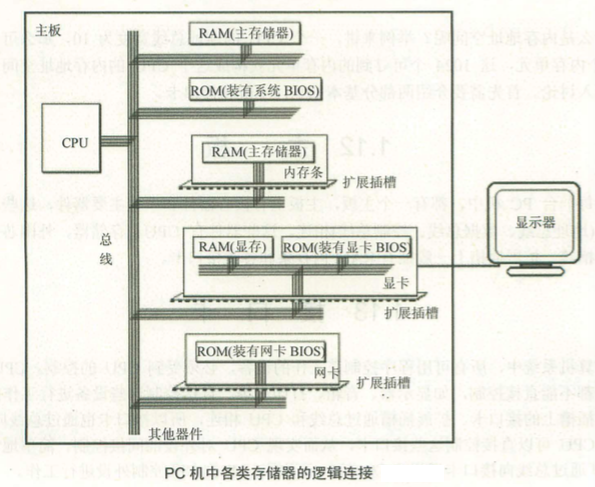
\includegraphics[width=3.7in]{slide01/images/PCLink}
\end{figure}
\end{frame}
